
\chapter{RL Basics}\label{rl_basics}
待重读的资源:
\begin{itemize}
%\setlength{\itemsep}{0pt}
%\setlength{\parsep}{0pt}
\setlength{\parskip}{0pt}
\item[-]
\url{https://yangyangfu.github.io/learning/reinforcement%20learning/2020/05/09/Bellman-Equation/}

\item[-]
\url{https://parkedphoton.com/bellman-equations/}

\item[-]
\url{https://inst.eecs.berkeley.edu/~cs188/sp10/slides/SP10%20cs188%20lecture%2011%20--%20reinforcement%20learning%20(6PP).pdf}
\end{itemize}


Reinforcement learning is useful when you have no training data or specific enough 
expertise about the problem. On a high level, you know WHAT you want, but not really 
HOW to get there. After all, not even Lee Sedol knows how to beat himself in Go.



\section{Value Functions}
% http://www.incompleteideas.net/book/ebook/node34.html

Almost all reinforcement learning algorithms are based on estimating value functions 
-- functions of states (or of state-action pairs) that estimate how good it is for 
the agent to be in a given state (or how good it is to perform a given action in a 
given state). The notion of "how good" here is defined in terms of future rewards 
that can be expected, or, to be precise, in terms of expected return. Of course the 
rewards the agent can expect to receive in the future depend on what actions it will 
take. Accordingly, value functions are defined with respect to particular policies.

Recall that a policy, $\pi$, is a mapping from each state, $s\in\mathcal{S}$, and 
action, $a\in\mathcal{A}(s)$, to the probability $\pi(s,a)$ of taking action $a$ 
when in state $s$. Informally, the value of a state $s$ under a policy $\pi$, denoted 
$V^\pi(s)$, is the expected return when starting in $s$ and following $\pi$ thereafter. 
For MDPs, we can define $V^\pi(s)$ formally as

\begin{equation}\label{rl-policy-state-value}
V^\pi(s) = \mathbb{E}_\pi\{R_t|s_t = s\} = 
\mathbb{E}_\pi\left\{ \sum_{k=0}^\infty\gamma^k r_{t+k+1} | s_t = s \right\},
\end{equation}
where $\mathbb{E}_\pi\{ \}$ denotes the expected value given that the agent follows 
policy $\pi$, and $t$ is any time step. Note that the value of the terminal state, if 
any, is always zero. We call the function $V^\pi$ the {\bf state-value function for 
policy $\pi$}.

Similarly, we define the value of taking action $a$ in state $s$ under a policy $\pi$, 
denoted $Q^\pi(s,a)$, as the expected return starting from $s$, taking the action $a$, 
and thereafter following policy $\pi$:

\begin{equation}\label{rl-policy-action-value}
Q^\pi(s, a) = \mathbb{E}_\pi\{R_t|s_t = s, a_t = a\} = 
\mathbb{E}_\pi\left\{ \sum_{k=0}^\infty\gamma^k r_{t+k+1} | s_t = s, a_t = a \right\},
\end{equation}
We call $Q^\pi$ the {\bf action-value function for policy $\pi$}.

The value functions $V^\pi$ and $Q^\pi$ can be estimated from experience. For example, 
if an agent follows policy $\pi$ and maintains an average, for each state encountered, 
of the actual returns that have followed that state, then the average will converge to 
the state's value, $V^\pi(s)$, as the number of times that state is encountered 
approaches infinity. If separate averages are kept for each action taken in a state, 
then these averages will similarly converge to the action values, $Q^\pi(s,a)$. We call 
estimation methods of this kind Monte Carlo methods because they involve averaging over 
many random samples of actual returns. These kinds of methods are presented in MC methods. 
Of course, if there are very many states, then it may not be practical to keep separate 
averages for each state individually. Instead, the agent would have to maintain $V^\pi$ 
and $Q^\pi$ as parameterized functions and adjust the parameters to better match the 
observed returns. This can also produce accurate estimates, although much depends on 
the nature of the parameterized function approximator.

\begin{emp_box}
需要用到的符号

A Markov Decision Process is a tuple $<\mathcal{S}, \mathcal{A}, \mathcal{P}, 
\mathcal{R}, \gamma>$
\begin{itemize}
%\setlength{\itemsep}{0pt}
%\setlength{\parsep}{0pt}
\setlength{\parskip}{0pt}
\item[-]
$\mathcal{S}$ is a set of states called state space

\item[-]
$\mathcal{A}$ is a set of actions called action space

\item[-]
$\mathcal{P}$ is a state transition probability matrix \\
$\mathcal{P}^a_{ss'}=P(S_{t+1}=s'|S_t=s,A_t=a)$

\item[-]
$\mathcal{R}$ is a reward function \\
$ \mathcal{R}^a_s=\mathbb{E}\left[R_{t+1}|S_t=s,A_t=a\right]$

\item[-]
$\gamma\in[0, 1]$ is a discount factor for future reward
\end{itemize}

\end{emp_box}

A fundamental property of value functions used throughout reinforcement learning and 
dynamic programming is that they satisfy particular recursive relationships. For any 
policy $\pi$ and any state $s$, the following consistency condition holds between the 
value of $s$ and the value of its possible successor states:
\begin{align} 
V^\pi(s)&\doteq \mathbb{E}_\pi \{R_t|s_t=s \} \notag \\
&=\mathbb{E}_\pi\left[\sum_{k=0}^\infty\gamma^k r_{t+k+1}|s_t=s\right] \notag \\
&=\mathbb{E}_\pi\left\{r_{t+1} + \gamma\sum_{k=0}^\infty\gamma^k r_{t+k+2}|s_t=s\right\} \notag \\
&=\sum_{a}\pi(s, a)\sum_{s'}\mathcal{P}_{ss'}^a\left[ \mathcal{R}_{ss'}^a + \gamma
\mathbb{E}_\pi\left\{ \sum_{k=0}^\infty\gamma^k r_{t+k+2}|s_{t+1}=s' \right\} \right] \notag \\
&=\sum_{a}\pi(s,a)\sum_{s'}\mathcal{P}_{ss'}^a\left[ \mathcal{R}_{ss'}^a + 
\gamma V^\pi(s')\right], \label{Bellman_equation_state_value_function_policy}
\end{align}
where it is implicit that the actions, $a$, are taken from the set $\mathcal{A}(s)$, 
and the next states, $s'$, are taken from the set $\mathcal{S}$, or from $\mathcal{S}^*$ 
in the case of an episodic problem. Equation (\ref{Bellman_equation_state_value_function_policy}) 
is the Bellman equation for $V^\pi$. It expresses a relationship between the value of 
a state and the values of its successor states. Think of looking ahead from one state 
to its possible successor states, as suggested by Figure \ref{fig:backup_diagrams_rl}a. 
Each open circle represents a state and each solid circle represents a state-action pair. 
Starting from state $s$, the root node at the top, the agent could take any of some set 
of actions -- three are shown in Figure \ref{fig:backup_diagrams_rl}a. From each of these, 
the environment could respond with one of several next states, $s'$, along with a reward, 
$r$. The Bellman equation (\ref{Bellman_equation_state_value_function_policy}) averages 
over all the possibilities, weighting each by its probability of occurring. It states 
that the value of the start state must equal the (discounted) value of the expected next 
state, plus the reward expected along the way.

\begin{figure}[!htb]
\centering
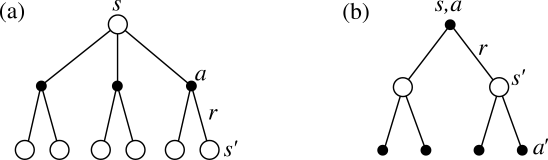
\includegraphics[scale=0.618]{pix/backup_diagrams_rl.png}
\caption{Backup diagrams for (a) $V^\pi$ and (b) $Q^\pi$.}
\label{fig:backup_diagrams_rl}
\end{figure}

The value function $V^\pi$ is the unique solution to its Bellman equation. We show in 
subsequent chapters how this Bellman equation forms the basis of a number of ways to 
compute, approximate, and learn $V^\pi$. We call diagrams like those shown in Figure 
\ref{fig:backup_diagrams_rl} backup diagrams because they diagram relationships that 
form the basis of the update or backup operations that are at the heart of 
reinforcement learning methods. These operations transfer value information back to a 
state (or a state-action pair) from its successor states (or state-action pairs). We 
use backup diagrams throughout the book to provide graphical summaries of the 
algorithms we discuss. (Note that unlike transition graphs, the state nodes of backup 
diagrams do not necessarily represent distinct states; for example, a state might be 
its own successor. We also omit explicit arrowheads because time always flows downward 
in a backup diagram.)


\subsection{Examples}


\subsubsection{Example: Gridworld}

Figure \ref{fig:grid_world}a uses a rectangular grid to illustrate value functions for 
a simple finite MDP. The cells of the grid correspond to the states of the environment. 
At each cell, four actions are possible: \colorbox{yellow}{north}, \colorbox{yellow}{south}, 
\colorbox{yellow}{east}, and \colorbox{yellow}{west}, which 
deterministically cause the agent to move one cell in the respective direction on the 
grid. Actions that would take the agent off the grid(处于边缘的格子移向方框外面的动作) 
leave its location unchanged, but also result in a reward of $-1$. Other actions result 
in a reward of $0$, except those that move the agent out of the special states $A$ and $B$. 
\colorbox{yellow}{From state $A$, all four actions yield a reward of $+10$ and take the 
agent to $A'$.} From state $B$, all actions yield a reward of $+5$ and take the agent to $B'$.

\begin{figure}[!htb]
\centering
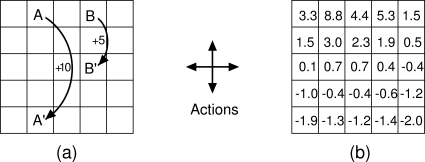
\includegraphics[scale=0.618]{pix/gridworld.png}
\caption{(a) exceptional reward dynamics; (b) state-value function for the equiprobable random policy.}
\label{fig:grid_world}
\end{figure}

\begin{emp_box}
上图中表b是按如下公式计算得出的:
\begin{align} 
V^\pi(s)=\sum_{a}\pi(s,a)\sum_{s'}\mathcal{P}_{ss'}^a\left[ \mathcal{R}_{ss'}^a + 
\gamma V^\pi(s')\right], \tag{\ref{Bellman_equation_state_value_function_policy}}
\end{align}
Recall that the policy $\pi$ is a mapping from each state $s\in\mathcal{S}$ and 
action $a\in\mathcal{A}(s)$ to the probability $\pi(s,a)$ of taking action $a$ 
when in state $s$. The state-value function $V^\pi(s)$ of a state $s$ under a 
policy $\pi$ is the expected return when starting in $s$ and following $\pi$ thereafter.
\end{emp_box}

Suppose the agent selects all four actions with equal probability in all states. Figure 
\ref{fig:grid_world}b shows the value function, $V^\pi$, for this policy, for the 
discounted reward case with $\gamma=0.9$. This value function was computed by solving 
the system of equations (\ref{Bellman_equation_state_value_function_policy}). Notice the 
negative values near the lower edge; these are the result of the high probability of 
hitting the edge of the grid there under the random policy. State A is the best state to 
be in under this policy, but its \textcolor{magenta}{expected return} is less than $10$, its 
\textcolor{magenta}{immediate reward}, 
because from $A$ the agent is taken to $A'$, from which it is likely to run into the edge 
of the grid. State $B$, on the other hand, is valued more than $5$, its immediate reward, 
because from $B$ the agent is taken to $B'$, which has a positive value. From $B'$ the 
expected penalty (negative reward) for possibly running into an edge is more than 
compensated for by the expected gain for possibly stumbling onto $A$ or $B$.


\subsection{Golf}

To formulate playing a hole of golf as a reinforcement learning task, we count a 
penalty (negative reward) of $-1$ for each stroke until we hit the ball into the hole. 
The state is the location of the ball. The value of a state is the negative of the 
number of strokes to the hole from that location. Our actions are how we aim and swing 
at the ball, of course, and which club we select. Let us take the former as given and 
consider just the choice of club, which we assume is either a putter or a driver. The 
upper part of Figure \ref{fig:golf} shows a possible state-value function, $V^{\text{putt}}$, 
for the policy that always uses the putter. The terminal state in-the-hole has a value of 
$0$. From anywhere on the green we assume we can make a putt; these states have value 
$-1$. Off the green we cannot reach the hole by putting, and the value is greater. If 
we can reach the green from a state by putting, then that state must have value one 
less than the green's value, that is, $-2$. For simplicity, let us assume we can putt 
very precisely and deterministically, but with a limited range. This gives us the sharp 
contour line labeled $-2$ in the figure; all locations between that line and the green 
require exactly two strokes to complete the hole. Similarly, any location within putting 
range of the $-2$ contour line must have a value of $-3$, and so on to get all the 
contour lines shown in the figure. Putting doesn't get us out of sand traps, so they 
have a value of $-\infty$. Overall, it takes us six strokes to get from the tee to the 
hole by putting.

\begin{figure}[!htb]
\centering
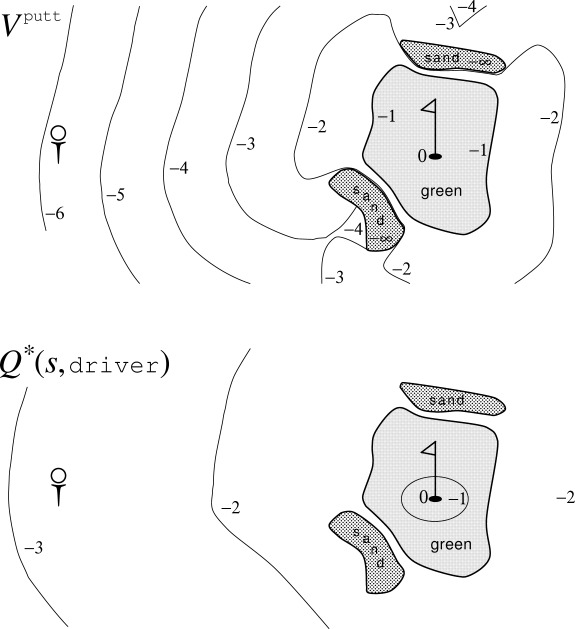
\includegraphics[scale=0.4]{pix/golf.png}
\caption{A golf example: the state-value function for putting (above) and the optimal action-value function for using the driver (below).}
\label{fig:golf}
\end{figure}

